\documentclass[ignorenonframetext,]{beamer}
\usetheme{Madrid}
\usecolortheme{whale}
\setbeamertemplate{caption}[numbered]
\setbeamertemplate{caption label separator}{:}
\setbeamercolor{caption name}{fg=normal text.fg}
\usepackage{amssymb,amsmath}
\usepackage{ifxetex,ifluatex}
\usepackage{fixltx2e} % provides \textsubscript
\usepackage{lmodern}
\ifxetex
  \usepackage{fontspec,xltxtra,xunicode}
  \defaultfontfeatures{Mapping=tex-text,Scale=MatchLowercase}
  \newcommand{\euro}{€}
\else
  \ifluatex
    \usepackage{fontspec}
    \defaultfontfeatures{Mapping=tex-text,Scale=MatchLowercase}
    \newcommand{\euro}{€}
  \else
    \usepackage[T1]{fontenc}
    \usepackage[utf8]{inputenc}
      \fi
\fi
% use upquote if available, for straight quotes in verbatim environments
\IfFileExists{upquote.sty}{\usepackage{upquote}}{}
% use microtype if available
\IfFileExists{microtype.sty}{\usepackage{microtype}}{}
\usepackage{longtable,booktabs}
\usepackage{caption}
% These lines are needed to make table captions work with longtable:
\makeatletter
\def\fnum@table{\tablename~\thetable}
\makeatother
\usepackage{graphicx}
\makeatletter
\def\maxwidth{\ifdim\Gin@nat@width>\linewidth\linewidth\else\Gin@nat@width\fi}
\def\maxheight{\ifdim\Gin@nat@height>\textheight0.8\textheight\else\Gin@nat@height\fi}
\makeatother
% Scale images if necessary, so that they will not overflow the page
% margins by default, and it is still possible to overwrite the defaults
% using explicit options in \includegraphics[width, height, ...]{}
\setkeys{Gin}{width=\maxwidth,height=\maxheight,keepaspectratio}

% Comment these out if you don't want a slide with just the
% part/section/subsection/subsubsection title:
\AtBeginPart{
  \let\insertpartnumber\relax
  \let\partname\relax
  \frame{\partpage}
}
\AtBeginSection{
  \let\insertsectionnumber\relax
  \let\sectionname\relax
  \frame{\sectionpage}
}
\AtBeginSubsection{
  \let\insertsubsectionnumber\relax
  \let\subsectionname\relax
  \frame{\subsectionpage}
}

\setlength{\parindent}{0pt}
\setlength{\parskip}{6pt plus 2pt minus 1pt}
\setlength{\emergencystretch}{3em}  % prevent overfull lines
\setcounter{secnumdepth}{0}
\usepackage[russian]{babel}
\author[Эконометрика. Лекция 10]{Эконометрика. Лекция 10}
\usepackage{dcolumn}
\DeclareMathOperator{\plim}{plim}
\newcommand{\e}{\varepsilon}
\newcommand{\hy}{\hat{y}}
\newcommand{\hb}{\hat{\beta}}

\title{Три сюжета напоследок}
\date{}

\begin{document}
\frame{\titlepage}

\begin{frame}{Три сюжета}

\begin{itemize}
\item
  Квантильная регрессия
\item
  Алгоритм случайного леса
\item
  Байесовский подход
\end{itemize}

\end{frame}

\begin{frame}{Квантильная регрессии}

Моделировать можно не только среднее, но и медиану или другой
определённый квантиль.

\end{frame}

\begin{frame}{Классическая регрессия --- модель для среднего}

Предпосылки классической модели:

\begin{itemize}
\item
  \(y_i=\beta_1 + \beta_2 x_i + \e_i\)
\item
  экзогенность, \(E(\e_i | x_i)=0\)
\item
  другие предпосылки
\end{itemize}

Следствие:

\[
E(y_i|x_i)=\beta_1 + \beta_2 x_i
\]

\end{frame}

\begin{frame}{Минимизация суммы квадратов}

Модель: \(E(y_i|x_i)=\beta_1 + \beta_2 x_i\)

\begin{itemize}
\item
  Сумма квадратов остатков, \(Q(\hb_1,\hb_2)=\sum_i (y_i - \hy_i)^2\)
\item
  Минимизируя \(Q(\hb_1,\hb_2)\) получаем состоятельные оценки
  \(\hb_1\), \(\hb_2\)
\end{itemize}

\end{frame}

\begin{frame}{Медианная регрессия}

Модель: \(Med(y_i|x_i)=\beta_1 + \beta_2 x_i\)

На большой выборке:

Математическое ожидание --- среднее арифметическое значение объясняемой
переменной \(y_i\) при заданном \(x_i\)

Медиана, \(Med(y_i|x_i)\) --- число, больше которого оказывается ровно
половина \(y_i\) при заданном \(x_i\)

\end{frame}

\begin{frame}{Алгоритм получения оценок}

\begin{itemize}
\item
  Сумма модулей остатков, \(M(\hb_1,\hb_2)=\sum_i |y_i - \hy_i|\)
\item
  Минимизируя \(M(\hb_1,\hb_2)\) получаем состоятельные оценки
  \(\hb_1\), \(\hb_2\)
\end{itemize}

\end{frame}

\begin{frame}{Пример у неоновой доски}

Найдите оценку \(\hb\) медианной регрессии: \[
Med(y_i|x_i)=\beta x_i
\]

Набор данных:

\begin{longtable}[c]{@{}cc@{}}
\toprule
\begin{minipage}[b]{0.05\columnwidth}\centering\strut
y
\strut\end{minipage} &
\begin{minipage}[b]{0.05\columnwidth}\centering\strut
x
\strut\end{minipage}\tabularnewline
\midrule
\endhead
\begin{minipage}[t]{0.05\columnwidth}\centering\strut
1
\strut\end{minipage} &
\begin{minipage}[t]{0.05\columnwidth}\centering\strut
1
\strut\end{minipage}\tabularnewline
\begin{minipage}[t]{0.05\columnwidth}\centering\strut
2
\strut\end{minipage} &
\begin{minipage}[t]{0.05\columnwidth}\centering\strut
5
\strut\end{minipage}\tabularnewline
\begin{minipage}[t]{0.05\columnwidth}\centering\strut
6
\strut\end{minipage} &
\begin{minipage}[t]{0.05\columnwidth}\centering\strut
5
\strut\end{minipage}\tabularnewline
\bottomrule
\end{longtable}

\end{frame}

\begin{frame}{Медианная и классическая регрессия}

\begin{itemize}
\item
  Классическая: от каких факторов зависит \(E(y_i|x_i)\)?
\item
  Медианная: от каких факторов зависит \(Med(y_i|x_i)\)?
\item
  Оценки \(\hat{\beta}_j\) и \(se(\hat{\beta}_j)\) считаются по разным
  формулам
\item
  Если распределение \(\e_i\) симметрично, то оба подхода дают
  асимптотически одинаковые оценки
\item
  Сходная проверка гипотез:
  \(t=\frac{\hat{\beta}_j-\beta_j}{se(\hat{\beta}_j)} \to N(0,1)\)
\end{itemize}

\end{frame}

\begin{frame}{Медианная регрессия: минусы}

\begin{itemize}
\item
  Нет явных формул для оценок коэффициентов и стандартных ошибок
\item
  Только асимптотические свойства оценок коэффициентов
\end{itemize}

\end{frame}

\begin{frame}{Медианная регрессия: плюсы}

\begin{itemize}
\item
  Взгляд на данные с другой стороны
\item
  Более устойчивые оценки в случае ``выбросов'' в \(\e_i\)
\end{itemize}

\end{frame}

\begin{frame}{Произвольная квантиль}

\begin{itemize}
\itemsep1pt\parskip0pt\parsep0pt
\item
  Медиана, \(Med(y_i)\), --- квантиль 50\%
\end{itemize}

\(P(y_i \leq Med(y_i))=0.5\)

\begin{itemize}
\itemsep1pt\parskip0pt\parsep0pt
\item
  Квантиль порядка \(\tau\), \(q_{\tau}\):
\end{itemize}

\(P(y_i \leq q_{\tau})=\tau\)

\begin{itemize}
\itemsep1pt\parskip0pt\parsep0pt
\item
  Например:
\end{itemize}

Квантиль порядка 10\% для \(y_i\) --- такое число \(q_{0.1}\), что
вероятность того, что \(y_i\) окажется меньше этого числа, равна 10\%.

\end{frame}

\begin{frame}{Квантильная регрессия}

Модель: \(q_{\tau}(y_i|x_i)=\beta_1^{\tau} + \beta_2^{\tau} x_i\)

\begin{itemize}
\itemsep1pt\parskip0pt\parsep0pt
\item
  Зависимость для разных квантилей может быть разная!
\end{itemize}

\end{frame}

\begin{frame}{Асимметричная сумма модулей остатков:}

\(M(\hb_1,\hb_2)=\sum_i w_i \cdot |y_i - \hy_i|\)

где веса \(w_i\) равны:

\[
w_i=\begin{cases}
(1-\tau), \; y_i < \hy_i \\
\tau, \; y_i \geq \hy_i \\
\end{cases}
\]

\begin{itemize}
\itemsep1pt\parskip0pt\parsep0pt
\item
  Минимизируя \(M(\hb_1,\hb_2)\) получаем состоятельные оценки
  \(\hb_1\), \(\hb_2\)
\end{itemize}

\end{frame}

\begin{frame}{Квантильная регрессия стоимости квартир}

недорогое жильё (10\%-ый квантиль):

\(\widehat{price}_i = 3.9 + 1.3 totsp_i\)

дорогое жильё (90\%-ый квантиль):

\(\widehat{price}_i = -102.4 + 3.6 totsp_i\)

\end{frame}

\begin{frame}{Квантильная регрессия стоимости на графике}

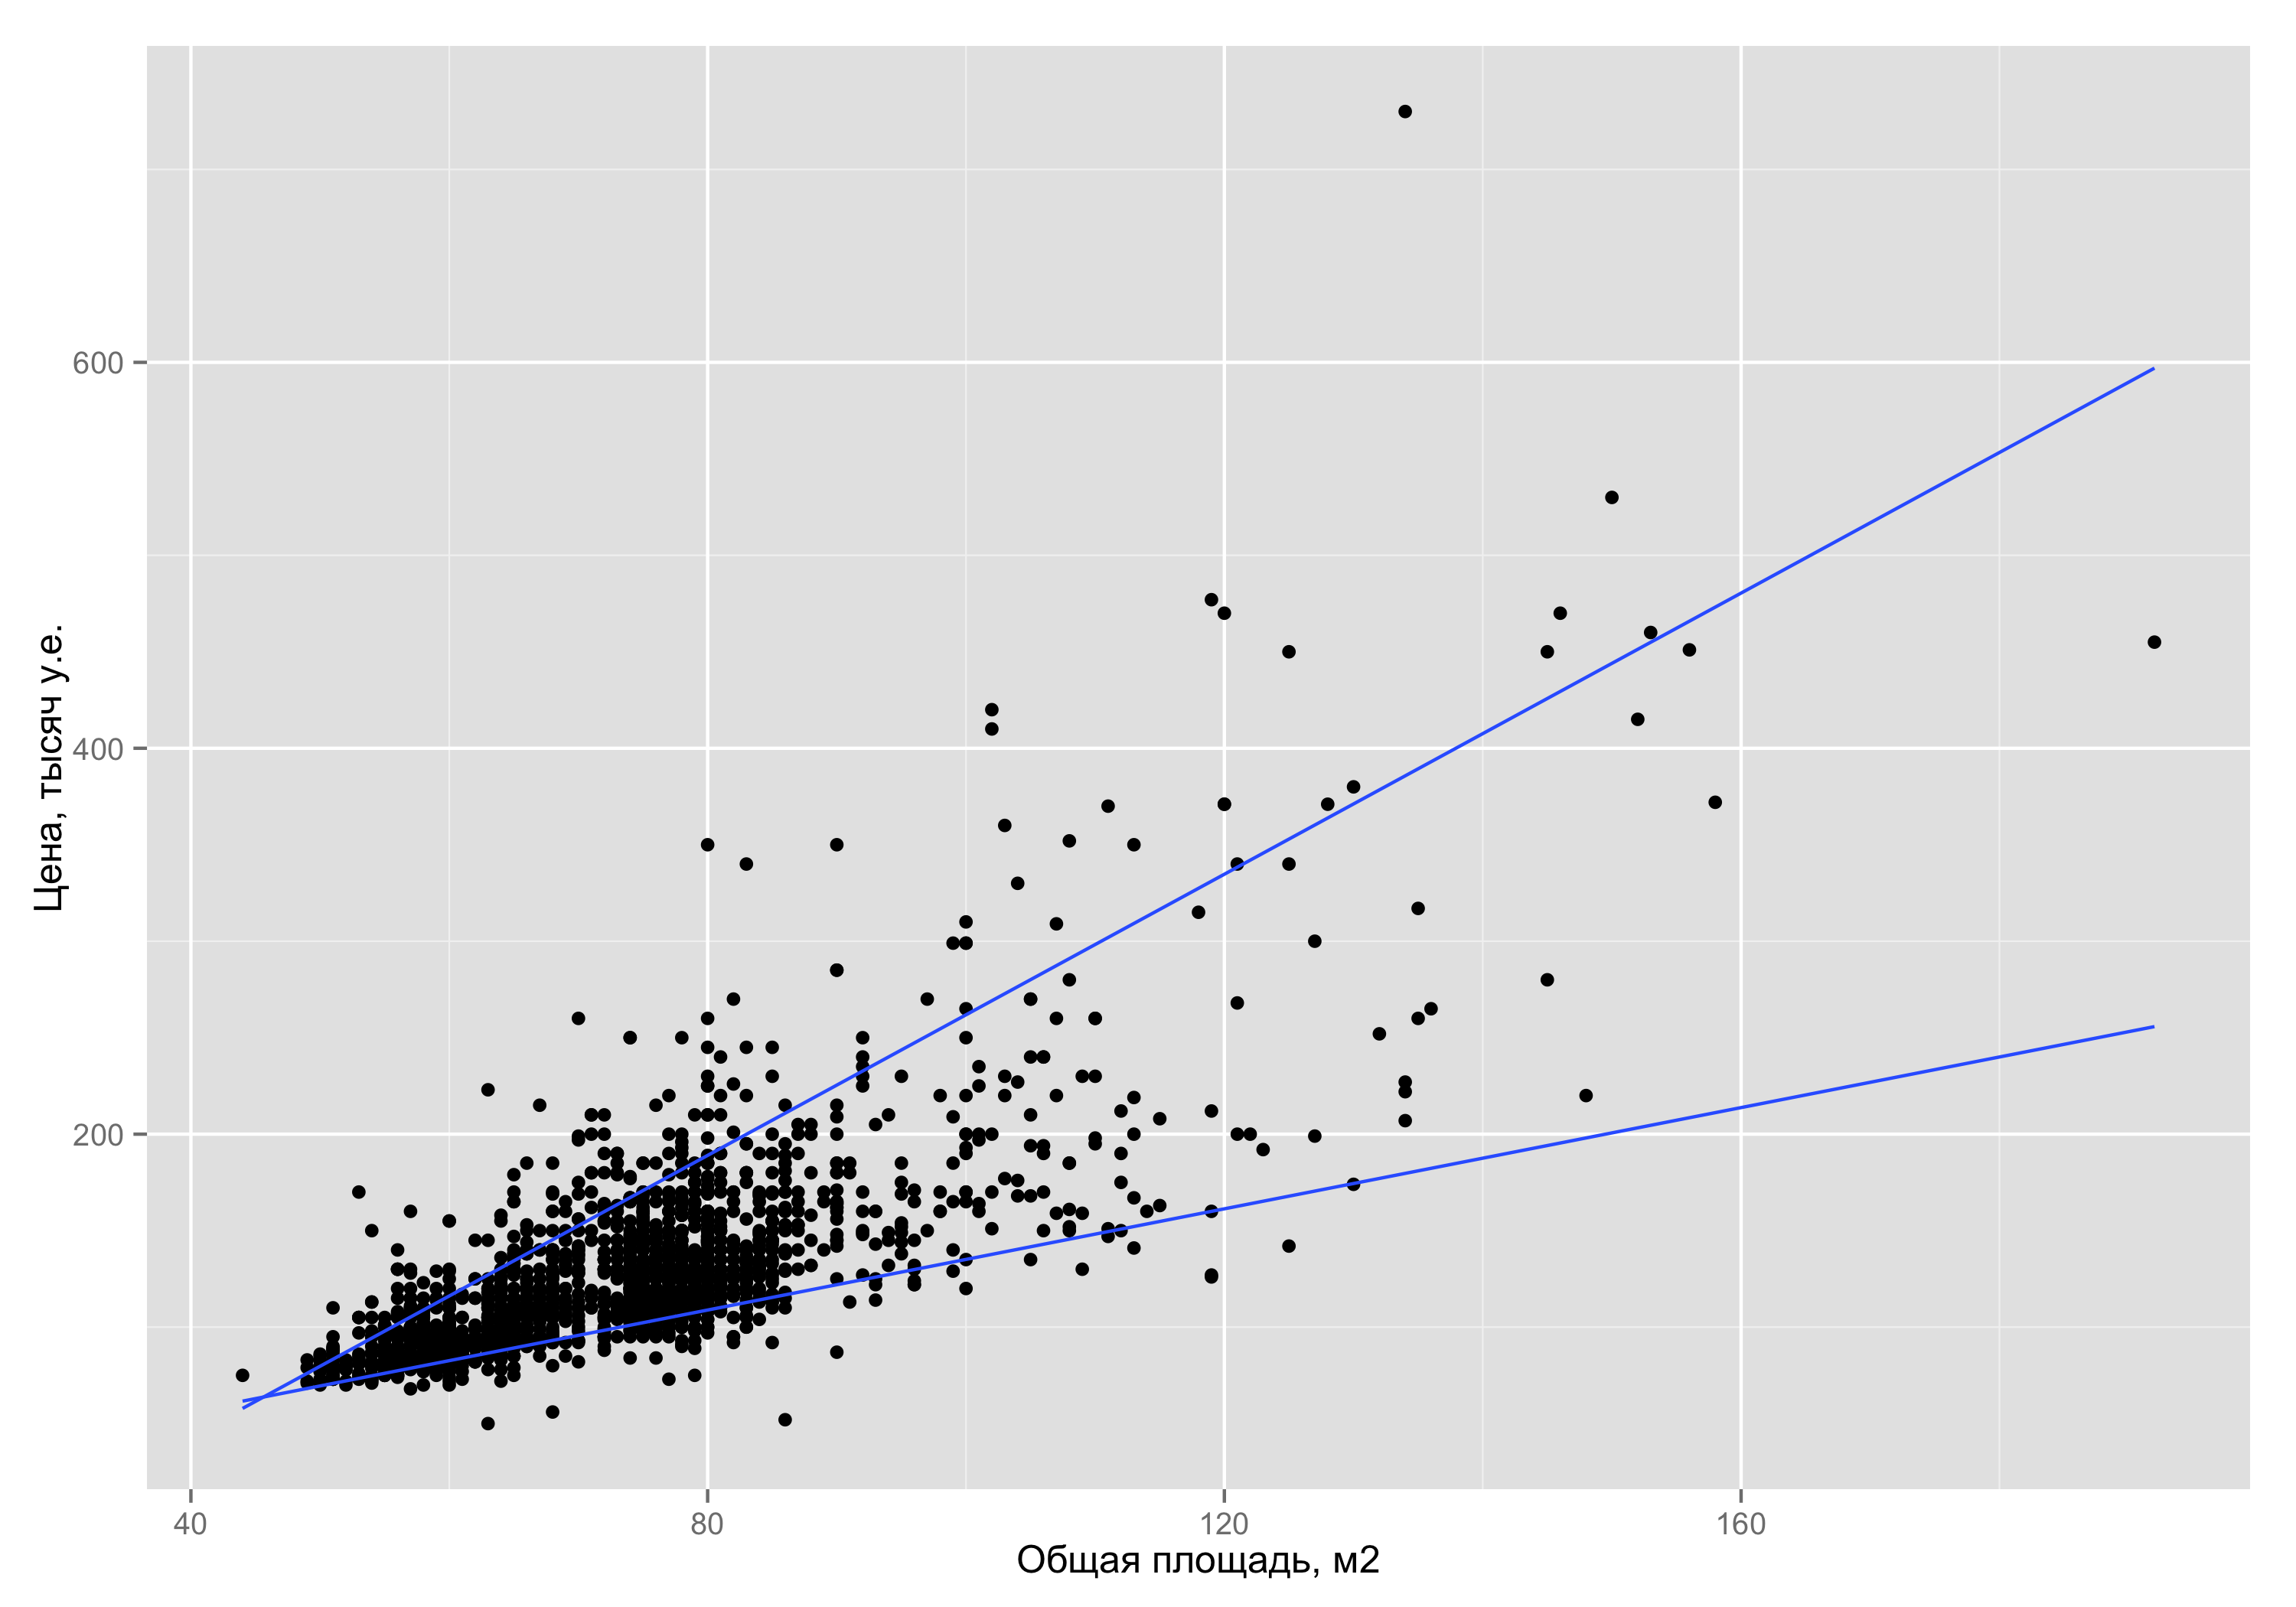
\includegraphics{base_q.png}

\end{frame}

\begin{frame}{Алгоритм случайного леса}

\begin{itemize}
\item
  Очень хорошо прогнозирует
\item
  Не объясняет, как устроены данные
\end{itemize}

\end{frame}

\begin{frame}{Две версии алгоритма}

\begin{itemize}
\item
  Для непрерывной \(y_i\)
\item
  Для качественной \(y_i\)
\end{itemize}

\end{frame}

\begin{frame}{Каждый мужчина должен посадить дерево}

Набор данных

\begin{longtable}[c]{@{}ccc@{}}
\toprule
\begin{minipage}[b]{0.05\columnwidth}\centering\strut
y
\strut\end{minipage} &
\begin{minipage}[b]{0.05\columnwidth}\centering\strut
x
\strut\end{minipage} &
\begin{minipage}[b]{0.05\columnwidth}\centering\strut
z
\strut\end{minipage}\tabularnewline
\midrule
\endhead
\begin{minipage}[t]{0.05\columnwidth}\centering\strut
1
\strut\end{minipage} &
\begin{minipage}[t]{0.05\columnwidth}\centering\strut
1
\strut\end{minipage} &
\begin{minipage}[t]{0.05\columnwidth}\centering\strut
-2
\strut\end{minipage}\tabularnewline
\begin{minipage}[t]{0.05\columnwidth}\centering\strut
1
\strut\end{minipage} &
\begin{minipage}[t]{0.05\columnwidth}\centering\strut
0
\strut\end{minipage} &
\begin{minipage}[t]{0.05\columnwidth}\centering\strut
3
\strut\end{minipage}\tabularnewline
\begin{minipage}[t]{0.05\columnwidth}\centering\strut
2
\strut\end{minipage} &
\begin{minipage}[t]{0.05\columnwidth}\centering\strut
0
\strut\end{minipage} &
\begin{minipage}[t]{0.05\columnwidth}\centering\strut
-4
\strut\end{minipage}\tabularnewline
\begin{minipage}[t]{0.05\columnwidth}\centering\strut
10
\strut\end{minipage} &
\begin{minipage}[t]{0.05\columnwidth}\centering\strut
0
\strut\end{minipage} &
\begin{minipage}[t]{0.05\columnwidth}\centering\strut
9
\strut\end{minipage}\tabularnewline
\begin{minipage}[t]{0.05\columnwidth}\centering\strut
20
\strut\end{minipage} &
\begin{minipage}[t]{0.05\columnwidth}\centering\strut
1
\strut\end{minipage} &
\begin{minipage}[t]{0.05\columnwidth}\centering\strut
9
\strut\end{minipage}\tabularnewline
\bottomrule
\end{longtable}

\end{frame}

\begin{frame}{Каждый мужчина должен посадить дерево}

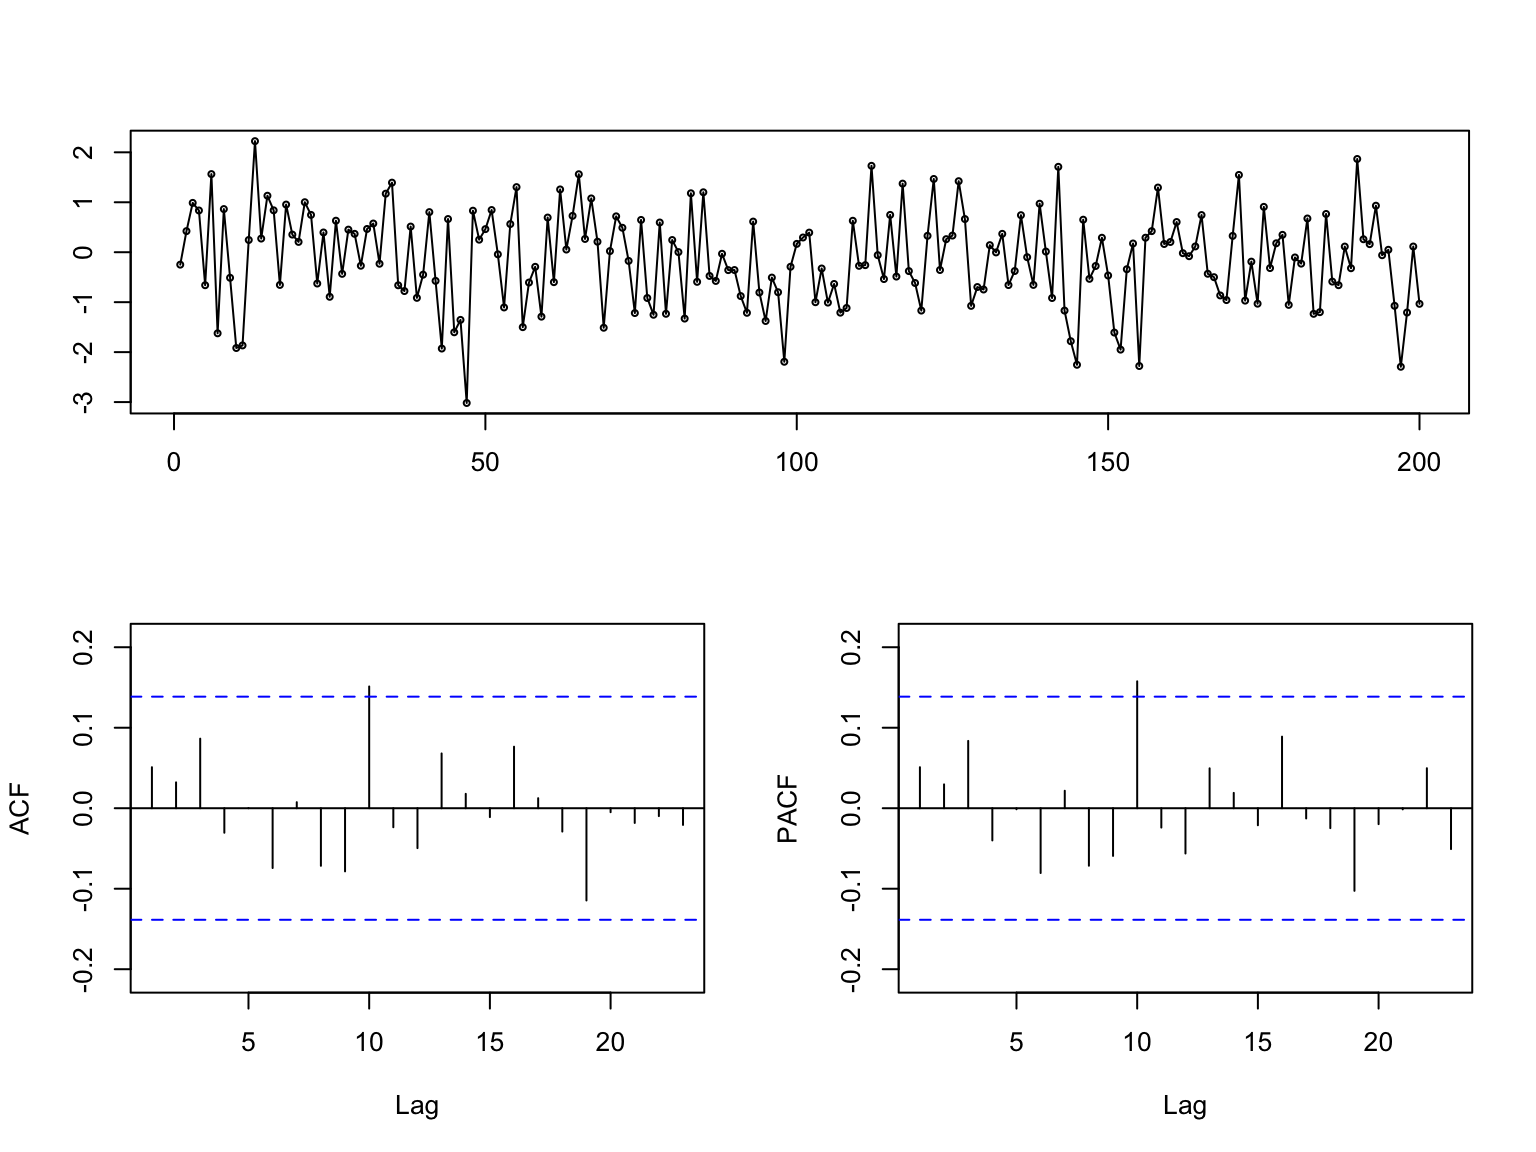
\includegraphics{lec_10_files/figure-beamer/unnamed-chunk-5-1.pdf}

\end{frame}

\begin{frame}{Как посадить дерево?}

\begin{itemize}
\item
  Из имеющихся \(k\) переменных случайно отбираем
  \(k'=\lceil k/3 \rceil\) переменных
\item
  Из отобранных \(k'\) переменных выбираем ту, которая даёт наилучшее
  деление ветви дерева на две
\item
  Повторяем до тех пор, пока в каждом терминальном узле остаётся больше
  \(nodesize=5\) наблюдений
\end{itemize}

\end{frame}

\begin{frame}{Наилучшее деление}

До деления: \(RSS=274.8\)

\(\{ 1, 1, 2, 10, 20\}\), \(\hy=\bar{y}=6.8\),

После разбиения: \(RSS=RSS_1+RSS_2=50.67\)

Слева: \(\{ 1, 1, 2 \}\), \(\hy=\bar{y}=1.33\), \(RSS_1=0.67\)

Справа: \(\{10,20\}\), \(\hy=\bar{y}=15\), \(RSS_2=50\)

\end{frame}

\begin{frame}{Алгоритм случайный}

Повторное применение алгоритма к тому же набору данных даст слегка
другие оценки

\end{frame}

\begin{frame}{Мужчина, владеющий R, может посадить целый лес!}

\begin{itemize}
\item
  Случайным образом отбираем (с повторениями) \(n\) наблюдений из
  исходных \(n\) наблюдений
\item
  Сажаем дерево по случайной подвыборке
\item
  Повторяем до получения \(n_{tree}=500\) деревьев
\end{itemize}

\end{frame}

\begin{frame}{Прогноз случайного леса:}

\begin{itemize}
\item
  Каждое из \(n_{tree}=500\) деревьев даёт свой прогноз \(\hy_i\)
\item
  Усредняем и получаем финальный прогноз
\end{itemize}

\end{frame}

\begin{frame}{Неоновая доска. Пример построения регрессионного дерева}

\begin{longtable}[c]{@{}cc@{}}
\toprule
\begin{minipage}[b]{0.05\columnwidth}\centering\strut
y
\strut\end{minipage} &
\begin{minipage}[b]{0.05\columnwidth}\centering\strut
x
\strut\end{minipage}\tabularnewline
\midrule
\endhead
\begin{minipage}[t]{0.05\columnwidth}\centering\strut
1
\strut\end{minipage} &
\begin{minipage}[t]{0.05\columnwidth}\centering\strut
1
\strut\end{minipage}\tabularnewline
\begin{minipage}[t]{0.05\columnwidth}\centering\strut
2
\strut\end{minipage} &
\begin{minipage}[t]{0.05\columnwidth}\centering\strut
2
\strut\end{minipage}\tabularnewline
\begin{minipage}[t]{0.05\columnwidth}\centering\strut
9
\strut\end{minipage} &
\begin{minipage}[t]{0.05\columnwidth}\centering\strut
3
\strut\end{minipage}\tabularnewline
\begin{minipage}[t]{0.05\columnwidth}\centering\strut
10
\strut\end{minipage} &
\begin{minipage}[t]{0.05\columnwidth}\centering\strut
4
\strut\end{minipage}\tabularnewline
\begin{minipage}[t]{0.05\columnwidth}\centering\strut
10
\strut\end{minipage} &
\begin{minipage}[t]{0.05\columnwidth}\centering\strut
5
\strut\end{minipage}\tabularnewline
\bottomrule
\end{longtable}

\end{frame}

\begin{frame}{Байесовский подход}

Опишем наше незнание параметра \(\theta\) в виде априорного закона
распределения!

\end{frame}

\begin{frame}{Пример. Неизвестная вероятность}

\begin{itemize}
\itemsep1pt\parskip0pt\parsep0pt
\item
  \(p \in [0;1]\)
\end{itemize}

Априорная плотность:

\[
f(p)=\begin{cases}
1, \; p\in[0;1] \\
0, \; \text{ иначе }
\end{cases}
\]

\end{frame}

\begin{frame}{Пример. Неизвестный положительный коэффициент}

\begin{itemize}
\itemsep1pt\parskip0pt\parsep0pt
\item
  \(\beta \in [0;+\infty)\)
\end{itemize}

Априорная плотность:

\[
f(\beta)=\begin{cases}
exp(-\beta), \; \beta \in[0;\infty) \\
0, \; \text{ иначе }
\end{cases}
\]

\end{frame}

\begin{frame}{Модель}

Модель задаёт закон распределения наблюдений, \(y_i\), при фиксированном
значении параметров

Например,

\[
y_i = \beta_1 + \beta_2 x_i + \e_i, \; \e_i \sim N(0,\sigma^2)
\]

\end{frame}

\begin{frame}{Кристально-чистая логика байесовского подхода}

Определяем:

\begin{itemize}
\item
  Априорное распределение, \(f(\theta)\)
\item
  Модель для данных, \(f(y|\theta)\)
\end{itemize}

По формуле условной вероятности получаем:

\begin{itemize}
\itemsep1pt\parskip0pt\parsep0pt
\item
  Апостериорное распределение, \(f(\theta|y)\)
\end{itemize}

\end{frame}

\begin{frame}{Формула условной вероятности}

\[
f(\theta|y)= \frac{f(y|\theta)\cdot f(\theta)}{f(y)} \sim f(y|\theta)\cdot f(\theta)
\]

\end{frame}

\begin{frame}{Пример у неоновой доски}

Наблюдения: пойманы 2 карася и щука.

Отдельные наблюдения независимы, вероятность поймать щуку и карася
стабильна во времени.

Найдите апостериорную плотность вероятности поймать карася в пруду.

\begin{itemize}
\item
  нет информации
\item
  Бабушка: караси встречаются чаще щук!
\end{itemize}

\end{frame}

\begin{frame}{Как описать сложную функцию плотности?}

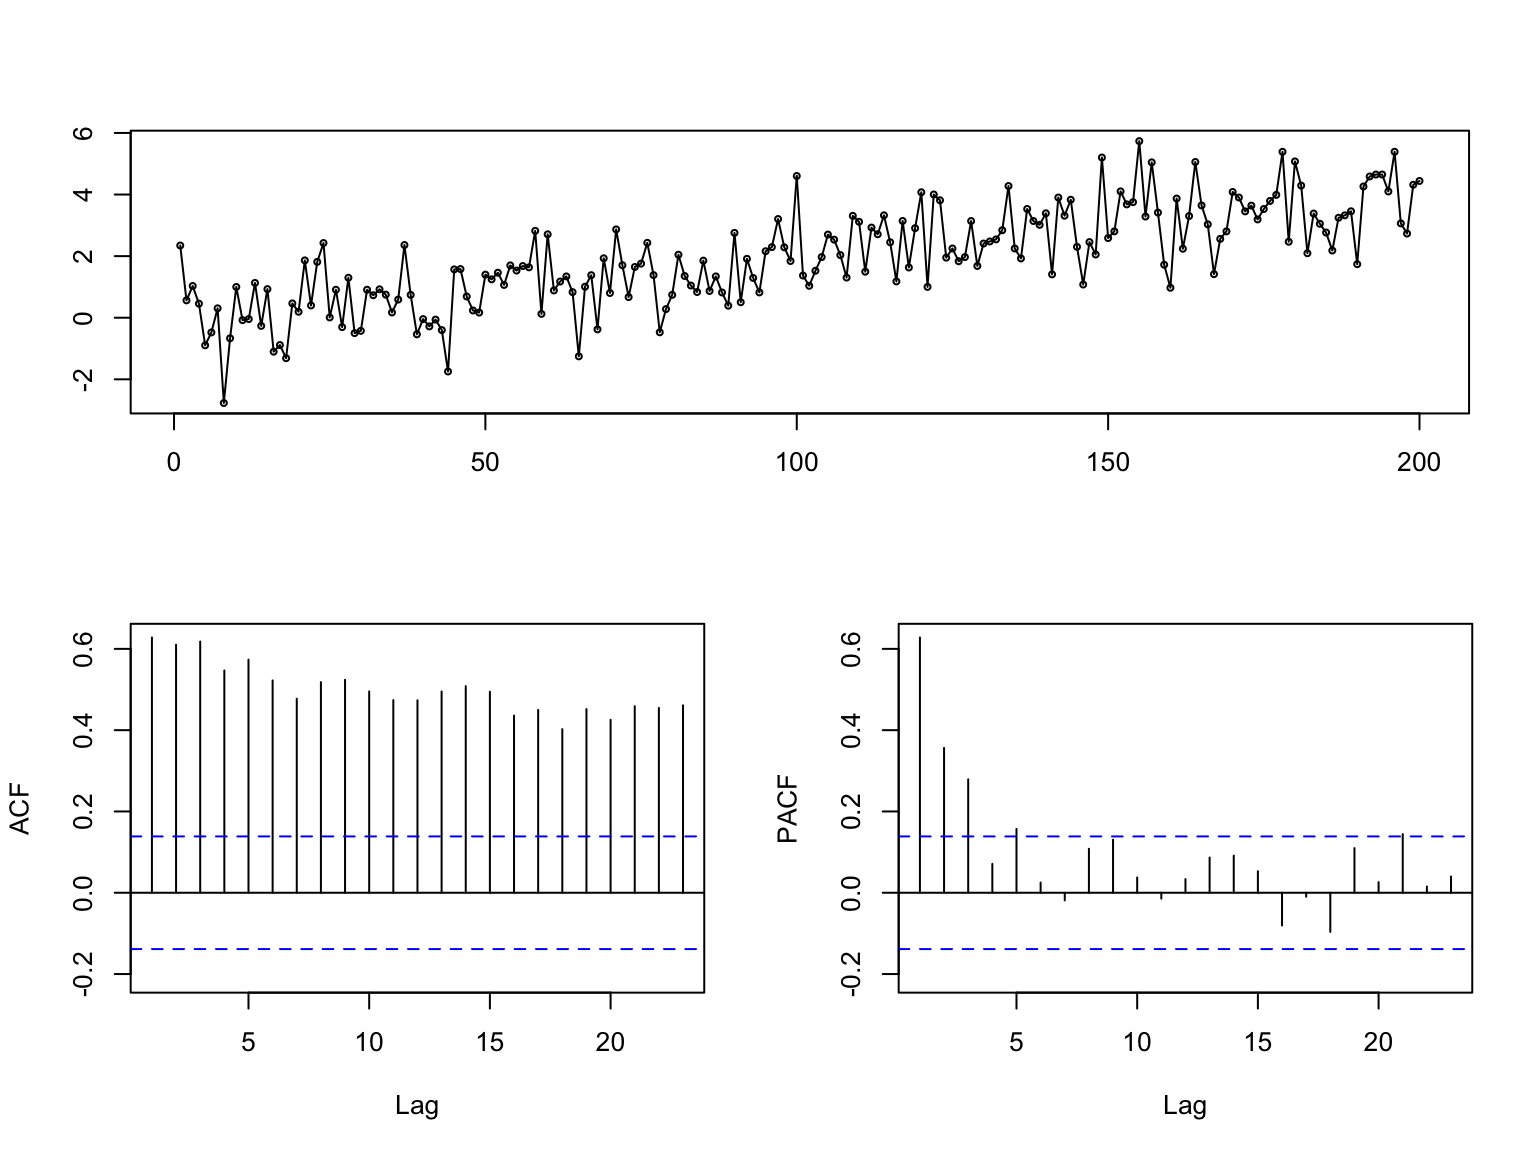
\includegraphics{lec_10_files/figure-beamer/unnamed-chunk-7-1.pdf}

\end{frame}

\begin{frame}{Сколь угодно точное описание любой плотности!}

\begin{itemize}
\itemsep1pt\parskip0pt\parsep0pt
\item
  Большая выборка независимых значений случайной величины \(r\):
\end{itemize}

\(r_1\), \(r_2\), \(r_3\), \ldots, \(r_{10000}\)

\begin{itemize}
\itemsep1pt\parskip0pt\parsep0pt
\item
  Можно оценить всё: \(E(r)\), \(E(r^2)\), \(P(r>0)\)
\end{itemize}

\end{frame}

\begin{frame}{Монте-Карло по схеме Марковской цепи}

MCMC (Markov Chain Monte Carlo)

Заменяет формулу условной вероятности

\end{frame}

\begin{frame}{Алгоритм MCMC}

На входе:

\begin{itemize}
\item
  Априорное распределение, \(f(\theta)\)
\item
  Модель для данных, \(f(y|\theta)\)
\end{itemize}

На выходе:

\begin{itemize}
\itemsep1pt\parskip0pt\parsep0pt
\item
  Большая выборка из апостериорного распределения, \(f(\theta|y)\)
\end{itemize}

\end{frame}

\begin{frame}{Алгоритм случайный}

Повторное применение алгоритма к тому же набору данных даст слегка
другие оценки

\end{frame}

\begin{frame}{Плюсы байесовского подхода}

\begin{itemize}
\itemsep1pt\parskip0pt\parsep0pt
\item
  Можно задавать вопросы про неизвестные параметры:
\end{itemize}

\(P(\beta_3 >0 | y)\), \(P(\beta_3=0 | y)\), \(E(\beta_3 | y)\)?

\begin{itemize}
\itemsep1pt\parskip0pt\parsep0pt
\item
  Апостериорное распределение есть всегда!
\end{itemize}

даже при жесткой мультиколлинеарности и полном отсутствии наблюдений

\end{frame}

\begin{frame}{Минусы байесовского подхода}

\begin{itemize}
\item
  Его не все знают
\item
  Может требовать больших объемов вычислений
\end{itemize}

\end{frame}

\begin{frame}{MCMC и логит}

``Идеальное прогнозирование'' --- ситуация, в которой ML оценки
логит-модели не существуют

\end{frame}

\begin{frame}{Логит-модель}

\(y_i \in \{0,1\}\).

\(y_i=\begin{cases} 1, y^*_i \geq 0 \\ 0, y^*_i <0 \end{cases}\)

Скрытая переменная: \(y^*_i=\beta_1 +\beta_2 x_i +\varepsilon_i\).

\end{frame}

\begin{frame}{Априорное распределение для логит модели}

\(\beta \sim N(b_0, B_0^{-1})\)

Гиперпараметры:

\(b_0\) --- априорное среднее

\(B_0\) --- априорная матрица точности

\(B_0^{-1}=Var(\beta)\)

\end{frame}

\begin{frame}{Выбор априорных гиперпараметров}

Традиционно:

\(b_0 = (0, 0, \ldots, 0)'\)

\(B_0 = \begin{pmatrix} d & 0 & 0 & \ldots \\ 0 & d & 0 & \ldots \\ 0 & 0 & d & \ldots \\ \vdots & \vdots & \vdots & \\ \end{pmatrix}\)

Число \(d\) мало

То есть: \(\beta_1 \sim N(0, 1/d)\), \(\beta_2 \sim N(0, 1/d)\),
\ldots{}

\end{frame}

\begin{frame}{Пример проблемной ситуации}

\begin{longtable}[c]{@{}cc@{}}
\toprule
\begin{minipage}[b]{0.05\columnwidth}\centering\strut
y
\strut\end{minipage} &
\begin{minipage}[b]{0.05\columnwidth}\centering\strut
x
\strut\end{minipage}\tabularnewline
\midrule
\endhead
\begin{minipage}[t]{0.05\columnwidth}\centering\strut
0
\strut\end{minipage} &
\begin{minipage}[t]{0.05\columnwidth}\centering\strut
1
\strut\end{minipage}\tabularnewline
\begin{minipage}[t]{0.05\columnwidth}\centering\strut
0
\strut\end{minipage} &
\begin{minipage}[t]{0.05\columnwidth}\centering\strut
2
\strut\end{minipage}\tabularnewline
\begin{minipage}[t]{0.05\columnwidth}\centering\strut
1
\strut\end{minipage} &
\begin{minipage}[t]{0.05\columnwidth}\centering\strut
3
\strut\end{minipage}\tabularnewline
\bottomrule
\end{longtable}

Логит и пробит оценки не существуют

\end{frame}

\begin{frame}{Логит со вкусом Байеса}

Априорно: \(\beta_1 \sim N(0, 10^2)\), \(\beta_2 \sim N(0, 10^2)\)

Апостериорные средние:

\(\hy_i^*=-10.8 + 4.5 x_i\)

\(y_i=\begin{cases} 1, y^*_i \geq 0 \\ 0, y^*_i <0 \end{cases}\)

\end{frame}

\begin{frame}{Регрессия пик-плато}

Модель: \(y_i = \beta_1 + \beta_2 x_i + \beta_3 z_i +\e_i\),
\(\e_i \sim N(0, \sigma^2)\)

\end{frame}

\begin{frame}{Вариант априорного распределения пик-плато}

\begin{itemize}
\item
  \(\beta_j | \gamma_j, \tau^2_j \sim N(0, \gamma_j \cdot \tau^2_j )\)
\item
  \(\gamma_j = \begin{cases} 1, \text{ с вероятностью } 1/2 \\ 0, \text{ с вероятностью } 1/2 \end{cases}\)
\item
  \(\tau_j^2 \sim \Gamma^{-1}(a_1,a_2)\)
\item
  \(\sigma^2 \sim \Gamma^{-1}(b_1,b_2)\)
\end{itemize}

Гиперпараметры: \(a_1\), \(a_2\), \(b_1\), \(b_2\)

\end{frame}

\begin{frame}{Регрессия пик-плато}

Позволяет напрямую отвечать на вопрос:

Чему равна вероятность \(P(\beta_2 = 0 | y)\)?

\end{frame}

\begin{frame}{Пример с машинами}

Апостериорные средние значения коэффициентов:

\(\widehat{dist}_i = 12.81 + 0.28 speed_i + 0.01 speed_i^2\)

Апостериорные вероятности:

\(P(\beta_{speed}=0 | y )=0.15\)

\(P(\beta_{speed^2}=0 | y )=0.05\)

\end{frame}

\begin{frame}{Большое спасибо}

Нам не удалось решить все наши задачи.

Решения, что мы находим, лишь ставят перед нами новые вопросы. В
каком-то смысле, мы также мало знаем, как и раньше. Но мы верим, что
наше незнание стало глубже, а не знаем мы всё более важные вещи.

Большое спасибо тем, кто прошел вместе с нами этот курс до конца!

\end{frame}

\end{document}
